 \sloppy
\begin{center}{\fontsize{16pt}{16pt}\selectfont \textbf{Python Object Oriented} \\}\end{center}


\begin{figure}[ht]
	\centerline{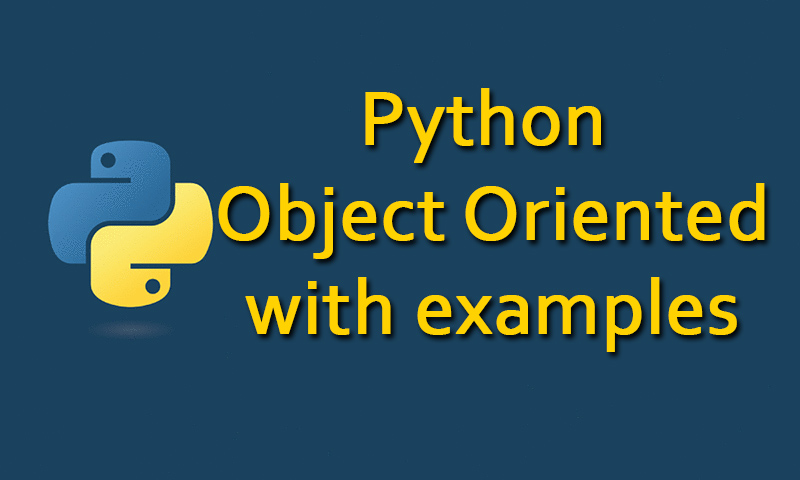
\includegraphics[width=0.70\textwidth]{Gambar/dapi3.jpg}}
	\caption{Python Object Oriented}
	\label{Python Object Oriented}
\end{figure}



\section {Pengertian }
\subsection {Python Object Oriented}

Phyton merupakan bahasa pemrograman yang berorientasi obyek dinamis, dapat digunakan untuk bermacam-macam pengembangan perangkat lunak. Phyton menyediakan dukungan yang kuat untuk integrasi dengan bahasa pemrograman lain dan alat-alat bantu lainnya.
Object Oriented Programming (OOP) adalah sebuah pendekatan pemrograman dimana objek didefinisikan dengan metode (fungsi, action, atau events) dan sifat (nilai serta karakteristik), sehingga mudah dibaca, lebih banyak kode yang dapat digunakan kembali.
Python telah menjadi bahasa berorientasi objek sejak itu ada. Karena itu, menciptakan dan menggunakan kelas dan objek sangat mudah. Bab ini membantu Anda menjadi ahli dalam menggunakan dukungan pemrograman berorientasi objek
Objek adalah sesuatu yang menamping nilai atau data dan dapat dikenakan operasi tertentu:
\begin {enumerate}
\item Class atau Kelas: adalah struktur data yang bisa digunakan untuk mendefinisikan objek yang menyimpan data bersama-sama nilai-nilai dan perilaku. Kelas adalah suatu entitas yang merupakan bentuk program dari suatu abstraksi untuk permasalahan dunia nyata, dan instans dari class merupakan realisasi dari beberapa objek.
\item Inheritace atau pewarisan merupakan konsep dalam pemrograman berbasis objek yang memungkinkan untuk membuat suatu kelas dengan didasarkan pada kelas yang sudah ada sehingga mewarisi semua method dan atributnya. Dengan cara seperti ini, semua method dan atribut yang terdapat pada kelas induk diturunkan ke kelas turunannya. Namun kelas turunannya dapat menambah method baru atau atribut baru tersendiri.
\item Method Constructor merupakan sebuah method yang akan otomatis dipanggil ketika objek diinstantiasi. Construktor umumnya digunakan untuk melakukan inisialisasi terhadap suatu variabel atau method.
\end {enumerate}

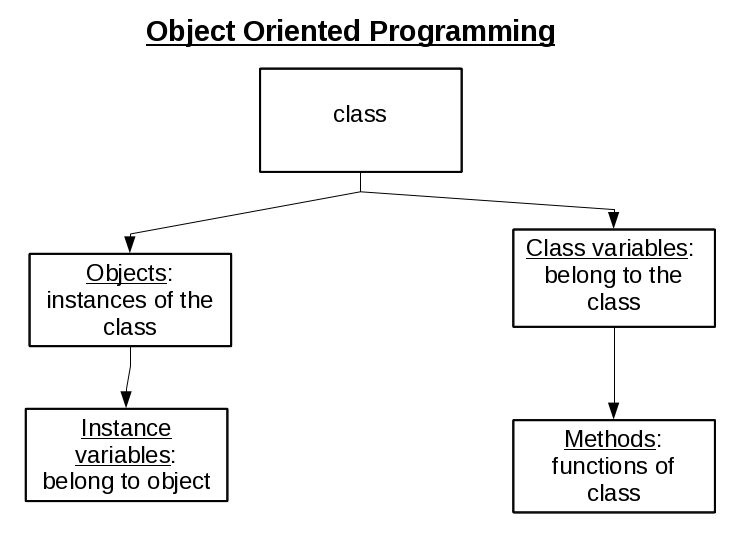
\includegraphics[width=10cm,height=7cm]{Gambar/dapi4.jpg}
\begin{equation}Python Object Oriented\end{equation}

Jika Anda tidak memiliki pengalaman sebelumnya dengan pemrograman berorientasi objek (OO), Anda mungkin  ingin berkonsultasi dengan kursus perkenalan atau setidaknya tutorial semacam itu sehingga Anda dapat memahami konsep dasarnya. Namun, di sini adalah pengenalan kecil Object-Oriented Programming (OOP) untuk membawa Anda pada kecepatan - Ikhtisar Terminologi OOP.

\begin {enumerate}
\item Kelas: Prototipe yang ditentukan pengguna untuk objek yang mendefinisikan seperangkat atribut yang menjadi ciri objek kelas apa pun. Atribut adalah data anggota (variabel kelas dan variabel contoh) dan metode, diakses melalui notasi titik.
\item Variabel kelas: Variabel yang dimiliki oleh semua instance kelas. Variabel kelas didefinisikan dalam kelas tapi di luar metode kelas manapun. Variabel kelas tidak digunakan sesering variabel contoh.
\item Anggota data: Variabel kelas atau variabel contoh yang menyimpan data yang terkait dengan kelas dan objeknya.
\item Fungsi overloading: Penugasan lebih dari satu perilaku ke fungsi tertentu. Operasi yang dilakukan bervariasi menurut jenis objek atau argumen yang terlibat.
\item Contoh variabel: Variabel yang didefinisikan di dalam metode dan hanya dimiliki oleh instance kelas saat ini.
\item Warisan: Pengalihan karakteristik kelas ke kelas lain yang berasal darinya. Contoh: Objek individual dari kelas tertentu. Obyek obj yang termasuk dalam Lingkaran kelas, misalnya, adalah turunan dari Lingkaran kelas.
\item Instansiasi: Pembuatan sebuah instance dari sebuah kelas.
\item Metode: Jenis fungsi khusus yang didefinisikan dalam definisi kelas.  
\item Objek: Contoh unik dari struktur data yang didefinisikan oleh kelasnya. Objek terdiri dari kedua anggota data (variabel kelas dan variabel contoh) dan metode.
\item Operator overloading: Penugasan lebih dari satu fungsi ke operator tertentu.
\end{enumerate}

Salah satu alasan yang paling penting untuk mempertimbangkan bekerja di OOP adalah bahwa ia menyediakan pendekatan pemodelan langsung dan memecahkan masalah didunia nyata.


\subsection {Membuat Kelas}

Pernyataan kelas membuat definisi kelas baru. Nama kelas segera mengikuti kelas kata kunci diikuti oleh titik dua sebagai berikut -

class ClassName:
~~ 'Optional class documentation string'
~~ class $  \_  $suite

Kelas memiliki kumpulan dokumentasi, yang bisa diakses melalui ClassName . $  \_  $ $  \_  $ doc $  \_  $ $  \_  $.  Class $  \_  $suite terdiri dari semua pernyataan komponen yang mendefinisikan anggota kelas, atribut dan fungsi data.


Berikut adalah contoh kelas Python sederhana -
\begin{verbatim}
class Employee:
~~ 'Common base class for all employees'
~~ empCount = 0

~~ def  $  \_  $ $  \_  $init $  \_  $ $  \_  $(self, name, salary):
~~~~~ self.name = name ~~~~~ self.salary = salary
~~~~~ Employee.empCount += 1
~~~~~ def displayCount(self):
~~~~~ print "Total Employee  $  \%  $d"  $  \%  $ Employee.empCount
~~ def displayEmployee(self):

~~~~~~print "Name : ", self.name,  ", Salary: ", self.salary
\end{verbatim}

\subsection{Variable empCount}
Variabel empCount adalah variabel kelas yang nilainya dibagi di antara semua contoh kelas ini. Ini bisa diakses sebagai Employee.empCount dari dalam kelas atau di luar kelas. Metode pertama  $  \_  $ $  \_  $init  $  \_  $ $  \_ $ () adalah metode khusus, yang disebut metode konstruktor kelas atau inisialisasi yang Python panggil saat Anda membuat instance baru dari kelas ini. Anda menyatakan metode kelas lain seperti fungsi normal dengan pengecualian bahwa argumen pertama untuk setiap metode adalah self. Python menambahkan argumen diri ke daftar untuk Anda; Anda tidak perlu memasukkannya saat Anda memanggil metode.


\subsection{Membuat Instance Objects}
Untuk membuat contoh kelas, Anda memanggil kelas menggunakan nama kelas dan meneruskan argumen apa pun yang diterima metode  $  \_  $ $  \_  $init $  \_  $ $  \_  $-nya.

"Ini akan menciptakan objek pertama kelas Karyawan"
Emp1 = Karyawan ("Zara", 2000)
"Ini akan menciptakan objek kedua dari kelas Karyawan"
Emp2 = Karyawan ("Manni", 5000)


\subsection{Mengakses Atribut}
Anda mengakses atribut objek menggunakan dot operator dengan objek. Variabel kelas akan diakses dengan menggunakan nama kelas sebagai berikut -

Emp1.displayEmployee ()
Emp2.displayEmployee (
Cetak "Jumlah Karyawan $  \%  $ d" $  \%  $ Employee.empCount

Sekarang, meletakkan semua konsep bersama -
\begin{verbatim}
 $  \#  $!/usr/bin/python
class Employee:
~~ 'Common base class for all employees'
~~ empCount = 0
~~ def  $  \_  $ $  \_  $init $  \_  $ $  \_  $(self, name, salary):
~~~~~ self.name = name
~~~~~ self.salary = salary
~~~~~ Employee.empCount += 1
~~ def displayCount(self):
~~~~ print "Total Employee  $  \%  $d"  $  \%  $ Employee.empCount
~~ def displayEmployee(self):
~~~~~~print "Name : ", self.name,  ", Salary: ", self.salary
"This would create first object of Employee class"
emp1 = Employee("Zara", 2000)
"This would create second object of Employee class"
emp2 = Employee("Manni", 5000)
emp1.displayEmployee()
emp2.displayEmployee()
print "Total Employee  $  \%  $d"  $  \%  $ Employee.empCount
\end{verbatim}
When the above code is executed, it produces the following result  \$ - \$

Name~:~ Zara ,Salary:  2000
Name~:~ Manni ,Salary:  5000
Total Employee 2
You can add, remove, or modify attributes of classes and objects at any time  \$ - \$
emp1.age~= 7  \ $  \#  $ Add an 'age' attribute.
emp1.age~= 8   \$  \#  $ Modify 'age' attribute.
del~emp1.age  \$  \#  $ Delete 'age' attribute.

Alih-alih menggunakan pernyataan normal untuk mengakses atribut, Anda dapat menggunakan fungsi berikut -

~~~ Getattr (obj, name [, default]): untuk mengakses atribut objek.

~~~ Hasattr (obj, name): untuk memeriksa apakah ada atribut atau tidak.


~~~ Setattr (obj, name, value): untuk mengatur atribut. Jika atribut tidak ada, maka akan dibuat.


~~~ The delattr (obj, name): untuk menghapus sebuah atribut.


Hasattr (emp1, 'age')  \$  \#  \$ Mengembalikan true jika atribut 'age' ada

Getattr (emp1, 'age')  \$  \#  \$ Mengembalikan nilai atribut 'age'

Setattr (emp1, 'age', 8)  \$  \#  \$ Set attribute 'age' di 8
\noindent
Delattr (empl, 'age')  \$  \#  \$ Hapus atribut 'umur'


Atribut Atribut Built-In

Setiap kelas Python terus mengikuti atribut bawaan dan mereka dapat diakses menggunakan operator dot seperti atribut lainnya -

\verb|~~~  $  \_  $ $  \_  $dict $  \_  $ $  \_  $|: Kamus yang berisi namespace kelas.

\verb|~~~  $  \_  $ $  \_  $doc $  \_  $ $  \_  $|: String dokumentasi kelas atau tidak, jika tidak terdefinisi.
\verb| ~~~  $  \_  $ $  \_  $name $  \_  $ $  \_  $|: nama kelas
\verb|~~~  $  \_  $ $  \_  $module $  \_  $ $  \_  $|: Nama modul dimana kelas didefinisikan. Atribut ini " $  \_  $ $  \_  $main $  \_  $ $  \_  $" dalam mode interaktif.
\verb|~~~  $  \_  $ $  \_  $bases $  \_  $ $  \_  $|: Tupel yang mungkin kosong yang berisi kelas dasar, sesuai urutan kejadiannya dalam daftar kelas dasar.

Untuk kelas di atas mari kita coba untuk mengakses semua atribut ini –
\begin{verbatim}
 $  \#  $!/usr/bin/python
class Employee:
~~ 'Common base class for all employees'
~~ empCount = 0
~~ def  $  \_  $ $  \_  $init $  \_  $ $  \_  $(self, name, salary):
~~~~~ self.name = name
~~~~~ self.salary = salary
~~~~~ Employee.empCount += 1
~~ def displayCount(self):
~~~~ print "Total Employee  $  \%  $d"  $  \%  $ Employee.empCount
~~ def displayEmployee(self): \par
~~~~~~print "Name : ", self.name,  ", Salary: ", self.salary
print "Employee. $  \_  $ $  \_  $doc $  \_  $ $  \_  $:", Employee. $  \_  $ $  \_  $doc $  \_  $ $  \_  $
print "Employee. $  \_  $ $  \_  $name $  \_  $ $  \_  $:", Employee. $  \_  $ $  \_  $name $  \_  $ $  \_  $
print "Employee. $  \_  $ $  \_  $module $  \_  $ $  \_  $:", Employee. $  \_  $ $  \_  $module $  \_  $ $  \_  $
print "Employee. $  \_  $ $  \_  $bases $  \_  $ $  \_  $:", Employee. $  \_  $ $  \_  $bases $  \_  $ $  \_  $
print "Employee. $  \_  $ $  \_  $dict $  \_  $ $  \_  $:", Employee. $  \_  $ $  \_  $dict $  \_  $ $  \_  $
\end{verbatim}

Bila kode diatas dieksekusi, maka menghasilkan hasil sebagai berikut -
Karyawan . \verb|$  \_  $ $  \_  $ doc $  \_  $ $  \_  $|: kelas dasar umum untuk semua karyawan
Karyawan . \verb|$  \_  $ $  \_  $ name $  \_  $ $  \_  $|: Karyawan
Karyawan . \verb|$  \_  $ $  \_  $ modul $  \_  $ $  \_  $|:  $  \_  $ $  \_  $main $  \_  $ $  \_  $
Karyawan . \verb|$  \_  $ $  \_  $ bases $  \_  $ $  \_  $|: ()
Karyawan . \verb|$  \_  $ $  \_  $ dict $  \_  $ $  \_  $|:  $  \{  $' $  \_  $ $  \_  $module $  \_  $ $  \_  $': ' $  \_  $ $  \_  $main $  \_  $ $  \_  $', 'displayCount':
<function displayCount at 0xb7c84994>, 'empCount': 2,
'DisplayEmployee': <function displayEmployee at 0xb7c8441c>,
\verb|' $  \_  $ $  \_  $doc $  \_  $ $  \_  $|': 'Kelas dasar umum untuk semua karyawan',
\verb|' $  \_  $ $  \_  $init $  \_  $ $  \_  $|': <function  $  \_  $ $  \_  $init $  \_  $ $  \_  $ di 0xb7c846bc> $  \}  $ \par

\subsection{Menghancurkan Objek (Pengumpulan Sampah)}
Python menghapus objek yang tidak dibutuhkan (tipe built-in atau instance kelas) secara otomatis untuk membebaskan ruang memori. Proses dimana Python secara berkala mengumpulkan kembali blok memori yang tidak lagi digunakan disebut Koleksi Sampah. Pengumpul sampah Python berjalan selama eksekusi program dan dipicu saat penghitungan referensi objek mencapai nol. Jumlah referensi referensi berubah karena jumlah alias yang menunjukkannya berubah. Jumlah referensi objek meningkat saat diberi nama baru atau ditempatkan dalam wadah (daftar, tupel, atau kamus). Jumlah referensi objek berkurang saat dihapus dengan del, rujukannya ditugaskan kembali, atau rujukannya tidak sesuai. Ketika penghitungan referensi objek mencapai nol, Python mengumpulkannya secara otomatis.
a = 40  \$  \#  \$ Buat objek <40>
B = a  \$  \#  \$ Tingkatkan ref. Hitung <40>
c = [b]  \$  \#  \$ Tingkatkan ref. Hitung <40>
Del  $  \#  $ Penurunan ref. Hitung <40>
b = 100  $  \#  $ Kurangi ref. Hitung <40>
C [0] = -1  $  \#  $ Kurangi ref. Hitung <40>

Anda biasanya tidak akan memperhatikan kapan pengumpul sampah menghancurkan contoh yatim piatu dan mengembalikan ruangnya. Tapi kelas bisa menerapkan metode khusus  $  \_  $ $  \_  $del  $  \_  $ $  \_ $ (), yang disebut destructor, yang dipanggil saat instance tersebut hendak dimusnahkan. Metode ini bisa digunakan untuk membersihkan sumber daya non memori yang digunakan oleh sebuah instance. \par

Contoh
Penghancur  \verb|$  \_  $ $  \_  $del  $  \_  $ $  \_  $| () ini mencetak nama kelas sebuah instance yang akan dihancurkan -
\begin{verbatim}
$  \#  $!/usr/bin/python
class Point:
~~ def  $  \_  $ $  \_  $init $  \_  $ $  \_  $( self, x=0, y=0):
~~~~~ self.x = x
~~~~~ self.y = y
~~ def  $  \_  $ $  \_  $del $  \_  $ $  \_  $(self):
~~~~~ class $  \_  $name = self. $  \_  $ $  \_  $class $  \_  $ $  \_  $. $  \_  $ $  \_  $name $  \_  $ $  \_  $
~~~~~ print class $  \_  $name, "destroyed"
pt1 = Point()
pt2 = pt1
pt3 = pt1
print id(pt1), id(pt2), id(pt3)  $  \#  $ prints the ids of the obejcts
del pt1
del pt2
del pt3
\end{verbatim}

\subsection{Kelas Warisan}
Alih-alih mulai dari nol, Anda dapat membuat kelas dengan menurunkannya dari kelas yang sudah ada sebelumnya dengan mencantumkan kelas induk dalam tanda kurung setelah nama kelas yang baru. Kelas anak mewarisi atribut kelas induknya, dan Anda dapat menggunakan atribut tersebut seolah-olah mereka didefinisikan di kelas anak. Kelas anak juga dapat mengesampingkan data anggota dan metode dari orang tua. Sintaksis Kelas turunan dinyatakan seperti kelas orang tua mereka; Namun, daftar kelas dasa yang diwarisi dari diberikan setelah nama kelas -

Kelas SubClassName (ParentClass1 [, ParentClass2, ...]):
\begin{verbatim}
~~ 'String dokumentasi kelas opsional'
~~ Class $  \_  $suite
 $  \#  $!/usr/bin/python

class~Parent:~~~~~~   $  \#  $ define parent class
~~ parentAttr = 100
~~ def  $  \_  $ $  \_  $init $  \_  $ $  \_  $(self):
~~~~~ print "Calling parent constructor"
~~ def parentMethod(self):
~~~~~ print 'Calling parent method'
~~ def setAttr(self, attr):
~~~~~ Parent.parentAttr = attr
~~ def getAttr(self):
~~~~~ print "Parent attribute :", Parent.parentAttr
class Child(Parent):  $  \#  $ define child class
~~ def  $  \_  $ $  \_  $init $  \_  $ $  \_  $(self):
~~~~~ print "Calling child constructor"
~~ def childMethod(self):
~~~~~ print 'Calling child method'
c~=~Child()~~~~~~~    $  \#  $ instance of child
c.childMethod()~~~~~  $  \#  $ child calls its method
c.parentMethod()~~~~  $  \#  $ calls parent's method
c.setAttr(200)~~~~~~  $  \#  $ again call parent's method
c.getAttr()~~~~~~~~~  $  \#  $ again call parent's method
Calling child constructor
Calling child method
Calling parent method
Parent attribute : 200
class~A:~~~~~~   $  \#  $ define your class A
.....
class~B:~~~~~~~   $  \#  $ define your class B
.....
class~C(A,~B):    $  \#  $ subclass of A and B
\end{verbatim}

Anda dapat menggunakan fungsi issubclass () atau isinstance () untuk memeriksa hubungan dua kelas dan contoh. Fungsi boolean issubclass (sub, sup) mengembalikan true jika sub subclass yang diberikan memang merupakan subclass dari superclass sup. The isinstance (obj, Class) fungsi boolean mengembalikan true jika obj adalah turunan dari Class Class atau merupakan instance dari subclass of Class.

\subsection{Metode utama}
Anda selalu dapat mengganti metode kelas induk Anda. Salah satu alasan untuk mengesampingkan metode orang tua adalah karena Anda mungkin menginginkan fungsi khusus atau berbeda di subkelas Anda. \par
Contoh
\begin{verbatim}
 $  \#  $! / Usr / bin / python
class parent:  $  \#  $ define parent class
~~ Def myMethod (diri):
~~~~~ Cetak 'metode induk panggilan'

Kelas anak (orang tua):  $  \#  $ define child class
~~ Def myMethod (diri):
~~~~~ Cetak 'metode memanggil anak'
C = Anak ()  $  \#  $ contoh anak
C.myMethod ()  $  \#  $ metode panggilan balik anak
\end{verbatim}
Bila kode diatas dieksekusi, maka menghasilkan hasil sebagai berikut -
Memanggil metode anak
Metode Base Overloading
Berikut daftar tabel beberapa fungsionalitas generik yang dapat Anda timpa di kelas Anda sendiri -

\subsection{Operator overloading}
Misalkan Anda telah membuat kelas Vektor untuk mewakili vektor dua dimensi, apa yang terjadi bila Anda menggunakan operator plus untuk menambahkannya? Kemungkinan besar Python akan berteriak pada Anda. Anda bisa, bagaimanapun, menentukan metode  $  \_  $ $  \_  $add $  \_  $ $  \_  $ di kelas Anda untuk melakukan penambahan vektor dan operator plus akan berperilaku sesuai harapan - \par
Contoh

\begin{verbatim}
 $  \# $! / Usr / bin / python
Kelas vektor:
~~ def  $  \_  $ $  \_  $init  $  \_  $ $  \_  $ (diri, a, b):
~~~~~ Self.a = a
~~~~~ Self.b = b
~~ def  $  \_  $ $  \_  $str  $  \_  $ $  \_  $ (diri):
~~~~~ Return 'Vector ( $  \%  $ d, $  \%  $ d)' $  \%  $ (self.a, self.b)
~~
~~ Def  $  \_  $ $  \_  $add  $  \_  $ $  \_  $ (diri sendiri, lainnya):
~~~~~ return Vector (self.a + other.a, self.b + other.b)
v1 = vektor (2,10)
v2 = vektor (5, -2)
cetak v1 + v2
\end{verbatim}

Bila kode diatas dieksekusi, maka menghasilkan hasil sebagai berikut -
Vektor (7,8)

\subsection{Persembunyian data}
Atribut objek mungkin atau mungkin tidak terlihat di luar definisi kelas. Anda perlu memberi nama atribut dengan awalan ganda ganda, dan atribut tersebut kemudian tidak langsung terlihat oleh orang luar.
Contoh

\begin {verbatim}
 $  \# $! / Usr / bin / python

Kelas JustCounter:
~~  $  \_  $ $  \_  $secretCount = 0
~
~~ def menghitung (diri):
~~~~~ self . $  \_  $ $  \_  $ secretCount + = 1
~~~~~ cetak diri . $  \_  $ $  \_  $ secretCount
counter = JustCounter ()
Counter.count ()
Counter.count ()
print counter . $  \_  $ $  \_  $ secretCount
\end{verbatim}

Bila kode diatas dieksekusi, maka menghasilkan hasil sebagai berikut -
1
2
Traceback (panggilan terakhir):
~ File "test.py", baris 12, di <module>
~~~ print counter . \verb|$  \_  $ $  \_  $| secretCount
AttributeError: instance JustCounter tidak memiliki atribut ' \verb|$  \_  $ $  \_  $|secretCount'

Python melindungi anggota tersebut dengan mengganti namanya secara internal untuk memasukkan nama kelas. Anda dapat mengakses atribut seperti object. $  \_  $className $  \_  $ $  \_  $attrName. Jika Anda akan mengganti baris terakhir Anda sebagai berikut, maka akan berhasil untuk Anda -
print counter. $  \_  $JustCounter $  \_  $ $  \_  $secretCount
Bila kode diatas dieksekusi, maka menghasilkan hasil sebagai berikut -
1
2
2
Contoh

Kelas bisa mewarisi kelas lainnya. Kelas dapat mewarisi atribut dan perilaku (metode) dari kelas lain, yang disebut kelas super. Sebuah kelas yang mewarisi dari kelas super disebut Sub-kelas. Kelas super kadang disebut nenek moyang juga. Ada hubungan hierarki antar kelas. Jika kita melihat lebih dekat contoh sebelumnya tentang akun kelas, kita dapat melihat bahwa model ini dapat memenuhi kebutuhan bank sebenarnya. Bank biasanya memiliki jenis akun yang berbeda, mis. Rekening Tabungan, Rekening Giro dan lain-lain. Meskipun jenis akun yang berbeda ini sangat berbeda, namun tetap memiliki banyak sifat dan metode yang sama. Misalnya. Setiap akun memiliki dan membutuhkan nomor rekening, pemegang dan saldo. Selanjutnya mungkin bagi masing-masing untuk menyetor atau menarik uang.
Jadi, ada sesuatu seperti akun "mendasar" darimana mereka mewarisi. Warisan digunakan untuk membuat kelas baru dengan menggunakan kelas yang ada. Yang baru dapat diciptakan dengan memperluas dan dengan membatasi kelas yang ada.
Sekarang saatnya untuk kembali ke Python dan melihat bagaimana kelas diimplementasikan dengan Python. Kita mulai dengan kelas yang paling sederhana, yang bisa didefinisikan. Kami hanya memberikan nama tapi menghilangkan semua spesifikasi lebih lanjut dengan menggunakan kata kunci n.
Class Account (objek):

Kami belum mendefinisikan atribut atau metode apa pun di kelas akun sederhana kami. Sekarang kita akan membuat sebuah instance dari kelas kosong ini:

>>> dari Account import Account
>>> x = Akun ()
>>> cetak x
<Account.Account objek di 0x7f364120ab90>
Sebuah metode berbeda dari satu fungsi saja dalam dua aspek:
Itu milik kelas dan itu didefinisikan dalam kelas
Parameter pertama dalam definisi suatu metode harus menjadi referensi "diri" pada instance kelas
Sebuah metode disebut tanpa parameter ini "diri"
Kami memperluas kelas kami dengan mendefinisikan beberapa metode. Tubuh dari metode ini masih belum ditentukan:
kelas Account (objek):
~~~ Transfer def (self, target, amount):
~~~~~~~ lulus
~~~ Def deposit (self, amount):
~~~~~~~ lulus
~~~ Def withdraw (self, amount):
~~~~~~~ lulus
~~~ def keseimbangan (diri):
~~~~~~~ lulus

Python tidak memiliki konstruktor eksplisit seperti C ++ atau Java, tapi metode \verb| $  \_  $ $  \_  $init  $  \_  $ $  \_  $ () dengan Python adalah sesuatu yang serupa, meskipun sebenarnya bukan konstruktor. Ini berperilaku dalam banyak hal seperti konstruktor, mis. Ini adalah kode pertama yang dijalankan, saat instance baru dari sebuah kelas dibuat. Nama itu terdengar seperti konstruktor " $  \_  $ $  \_  $init $  \_  $ $  \_  $|". Tapi secara tegas, akan salah jika menyebutnya sebagai konstruktor, karena contoh baru sudah "dibangun" pada saat metode  \verb|$  \_  $ $  \_  $init $  \_  $ $  \_  $ dipanggil. Tapi bagaimanapun, metode  $  \_  $ $  \_  $init $  \_  $ $  \_  $| digunakan - seperti konstruktor pada bahasa pemrograman berorientasi objek lainnya - untuk menginisialisasi variabel instance dari sebuah objek. Definisi metode init terlihat seperti definisi metode lainnya:

Def  \verb|$  \_  $ $  \_  $init  $  \_  $ $  \_  $| (self, holder, number, balance, credit \$  \_  \$line = 1500): 
~~~~~~~ self.Holder = pemegang
~~~~~~~ Nomor self.Number =
~~~~~~~ self.Balance = keseimbangan
~~~~~~~ self.CreditLine = credit \$  \_  \$line

Apa yang kami katakan tentang konstruktor berlaku bagi penghancur juga. Tidak ada destruktor "nyata", tapi ada yang serupa, yaitu metode  $  \_  $ $  \_  $del $  \_  $ $  \_  $. Hal ini disebut ketika contoh ini akan hancur. Jika kelas dasar memiliki metode  $  \_  $ $  \_  $del  $  \_  $ $  \_  $ (), metode  $  \_  $ $  \_  $del  $  \_  $ $  \_  $ () kelas turunan, jika ada, harus secara eksplisit memanggilnya untuk memastikan penghapusan komponen kelas dasar contoh yang tepat.
Contoh berikut menunjukkan kelas dengan konstruktor dan destruktor:

\begin{verbatim}
Kelas Salam:
~~~ Def  $  \_  $ $  \_  $init  $  \_  $ $  \_  $ (diri, nama):
~~~~~~~ self.name = nama
~~~ Def  $  \_  $ $  \_  $del  $  \_  $ $  \_  $ (diri):
~~~~~~~ Cetak "Destructor dimulai"
~~~ Def SayHello (diri):
~~~~~~~ Cetak "Halo", self.name
\end{verbatim}
